\documentclass[conference]{IEEEtran}
\IEEEoverridecommandlockouts
\usepackage{cite}
\usepackage{amsmath,amssymb,amsfonts}
\usepackage{algorithmic}
\usepackage{graphicx}
\usepackage{textcomp}
\usepackage{xcolor}
\usepackage{booktabs}
\usepackage{multirow}
\usepackage{url}

\def\BibTeX{{\rm B\kern-.05em{\sc i\kern-.025em b}\kern-.08em
    T\kern-.1667em\lower.7ex\hbox{E}\kern-.125emX}}

\begin{document}

\title{ECG Arrhythmia Classification Using Advanced Temporal Pattern Recognition}

\author{
\IEEEauthorblockN{Author Name\textsuperscript{1}}
\IEEEauthorblockA{
\textit{Department Name (TODO)} \\
\textit{Institution Name (TODO)} \\
City, Country (TODO) \\
email@domain.tld (TODO)}
}

\maketitle

\begin{abstract}
Cardiac arrhythmias are a leading indicator of life-threatening heart
conditions, and automated electrocardiogram (ECG) analysis is central to
scalable cardiac monitoring. Reliable automated classification remains
difficult because of severe class imbalance, inter-patient morphological
variability, and the risk of over-optimistic evaluation when beats from the
same patient leak between training and test sets. This paper presents a
controlled comparison of three heartbeat classification pipelines trained
and evaluated under an identical, patient-independent protocol on the
MIT-BIH Arrhythmia Database: (1) RR-interval and heart-rate-variability
(HRV) features with a Support Vector Machine (SVM); (2) Discrete Wavelet
Transform (DWT, Daubechies-4) coefficient statistics with a Random Forest;
and (3) a compact one-dimensional Convolutional Neural Network combined
with a Bidirectional Long Short-Term Memory network (1D-CNN+BiLSTM) trained
end-to-end on raw beat waveforms. All three models use the de Chazal
DS1/DS2 inter-patient split (44 of 48 records, 100{,}692 segmented beats)
and the AAMI EC57 five-class scheme (N, S, V, F, Q). On the held-out DS2
test set (49{,}691 beats), the Random Forest achieved the highest accuracy
(0.884) and weighted-F1 (0.882), the SVM achieved the highest macro-F1
(0.362) and ROC-AUC (0.812), and the CNN-BiLSTM, in this compact,
briefly-trained configuration, underperformed both classical approaches
(accuracy 0.449, macro-F1 0.183). The results show that hand-crafted,
patient-invariant features (RR timing in particular) generalise across
unseen patients more robustly than an intentionally small raw-waveform deep
model trained with limited compute, and that accuracy alone is a misleading
metric under the dataset's severe class imbalance. All results are
reported from executed experiments; no numbers in this paper are
simulated or assumed.
\end{abstract}

\begin{IEEEkeywords}
ECG, Arrhythmia Classification, Biomedical Signal Processing, Heart Rate
Variability, Discrete Wavelet Transform, Support Vector Machine, Random
Forest, Convolutional Neural Network, Bidirectional LSTM, Inter-Patient
Evaluation
\end{IEEEkeywords}

\section{Introduction}

The electrocardiogram (ECG) is the primary non-invasive signal used to
assess cardiac electrical activity, and automated identification of
abnormal heartbeats within it underlies a large share of modern cardiac
monitoring, from Holter analysis to wearable devices. An arrhythmia --- a
deviation from normal sinus rhythm --- can be a benign variant or a marker
of a serious underlying condition, so distinguishing the clinically
important categories of abnormal beats from normal ones, reliably and at
scale, is a long-standing pattern recognition problem.

Automated ECG beat classification is harder than it first appears, for
three compounding reasons. First, \textit{class imbalance} is severe:
normal beats vastly outnumber ectopic and fusion beats in any realistic
recording, so a classifier that is accurate on average can still be
clinically useless if it never recognises the rare, important classes.
Second, \textit{morphological variation across patients} is substantial --
the same arrhythmia can look different in two individuals due to anatomy,
lead placement, and baseline physiology, which means a model can appear
highly accurate yet fail to generalise if it is allowed to see a patient's
beats during training. Third, \textit{temporal dependency} matters: some
arrhythmia classes (e.g. premature beats) are defined largely by their
timing relative to neighbouring beats rather than by waveform shape alone,
while others are primarily morphological. These three issues motivate
comparing approaches that emphasise different information: beat timing,
frequency-domain morphology, and raw learned representations.

\textit{Research objective.} This paper does not propose a new algorithm;
its contribution is a controlled, leak-free comparison of three
representative and widely used families of ECG classification approaches
under one shared, reproducible experimental protocol, so that differences
in reported performance can be attributed to the modelling approach rather
than to inconsistencies in data handling. Concretely, we:
\begin{itemize}
\item implement and train (i) RR/HRV features with an SVM, (ii) DWT
  coefficient statistics with a Random Forest, and (iii) a 1D-CNN+BiLSTM
  trained on raw beat waveforms, on \emph{identical} preprocessed beats;
\item apply a genuine patient-independent (inter-patient) train/test split
  of the MIT-BIH Arrhythmia Database, so that no patient's beats appear in
  both sets, and restrict all hyperparameter tuning to the training
  partition;
\item report accuracy alongside macro-averaged and per-class metrics,
  which is necessary given the dataset's roughly 89\%-normal class
  imbalance; and
\item discuss, with evidence from the actual confusion matrices, why the
  three approaches disagree, rather than presenting a single
  aggregate ranking.
\end{itemize}

The remainder of this paper is organised as follows. Section~II reviews
related work in RR/HRV-based, wavelet-based, and deep-learning-based ECG
classification. Section~III describes the MIT-BIH dataset, the AAMI
class mapping, and the patient-independent split. Section~IV details the
preprocessing pipeline and the three modelling approaches. Section~V
reports the experimental results. Section~VI discusses the findings and
their implications, and Section~VII concludes with limitations and future
work.

\section{Related Work}

\textbf{RR-interval and HRV-based classification.} Because premature and
ectopic beats are frequently marked by abnormal timing relative to
neighbouring beats, several works have classified arrhythmias from RR
interval sequences alone. Tsipouras et al.~\cite{tsipouras2005arrhythmia}
built an arrhythmia classification system directly from the RR-interval
signal, demonstrating that timing information carries substantial
discriminative power even without waveform morphology. SVM classifiers in
particular have been applied to ECG arrhythmia features in several
studies, including Kohli et al.~\cite{kohli2010svm}, who evaluated
SVM-based methods for arrhythmia classification on ECG recordings.

\textbf{Wavelet-based morphological features.} The Discrete Wavelet
Transform (DWT) decomposes a signal into localized time-frequency bands,
which is well suited to the QRS complex's non-stationary, multi-scale
structure. Alickovic and Subasi~\cite{alickovic2016medical} combined DWT
feature extraction with a Random Forest classifier for heart arrhythmia
diagnosis, reporting that wavelet-domain statistical features are
effective inputs to ensemble tree classifiers -- the same combination
(DWT + Random Forest) adopted as Approach 2 in this paper, enabling a
direct methodological comparison.

\textbf{Deep learning for ECG classification.} More recent work replaces
hand-crafted features with representations learned directly from the
waveform. Acharya et al.~\cite{acharya2017deep} trained a deep
convolutional neural network to classify heartbeats directly from ECG
segments, showing that convolutional filters can learn discriminative
morphological patterns without explicit feature engineering. Hybrid
architectures that add a recurrent component to capture longer temporal
context have also been explored: Liu et al.~\cite{liu2019attention}
proposed an attention-based hybrid LSTM-CNN model for arrhythmia
classification on MIT-BIH, reporting high accuracy under their training
protocol. These works motivate Approach 3 in this paper, though -- as
Section~V shows -- the specific compact architecture and limited training
budget used here does not reproduce such high numbers, which is itself a
relevant and honestly reported finding (Section~VI).

\textbf{Evaluation protocol and the research gap.} A recurring
methodological concern across this literature is how the data is split.
de Chazal et al.~\cite{dechazal2004automatic} established the
widely-adopted inter-patient DS1/DS2 split of MIT-BIH specifically to
prevent a model from being evaluated on beats from patients it was trained
on, which otherwise substantially inflates reported accuracy. Many
subsequent papers evaluate only one modelling family under this protocol,
or compare families evaluated under different, not-directly-comparable
protocols. The gap this paper addresses is a same-protocol, same-data,
three-family comparison -- RR/HRV, DWT, and raw-waveform deep learning --
so that the reported differences reflect the modelling approach and not
inconsistent experimental setup.

\section{Dataset and Problem Formulation}

\subsection{MIT-BIH Arrhythmia Database}

This study uses the MIT-BIH Arrhythmia
Database~\cite{moody2001impact,goldberger2000physiobank}, distributed via
PhysioNet (\url{https://physionet.org/content/mitdb/1.0.0/}). It contains
48 half-hour, two-lead ambulatory ECG recordings sampled at 360~Hz with
11-bit resolution over a $\pm$5~mV range, collected by the Beth Israel
Hospital Arrhythmia Laboratory, together with cardiologist-verified
beat-by-beat annotations (a symbol and sample index for every heartbeat).

\subsection{Record Selection and Patient-Independent Split}

This project uses \textbf{44 of the 48 records}. Four records --
102, 104, 107, and 217 -- are excluded because they are dominated by
paced beats, which would otherwise distort both the normal-rhythm classes
and the already small unknown/paced class under the mapping used below;
excluding them is standard practice in the inter-patient MIT-BIH
literature~\cite{dechazal2004automatic}.

Beats are split by \emph{patient (record)}, never by individual beat,
following the de Chazal DS1/DS2
protocol~\cite{dechazal2004automatic}:
\begin{itemize}
\item \textbf{DS1 (train, 22 records):} 101, 106, 108, 109, 112, 114, 115,
  116, 118, 119, 122, 124, 201, 203, 205, 207, 208, 209, 215, 220, 223, 230.
\item \textbf{DS2 (test, 22 records):} 100, 103, 105, 111, 113, 117, 121,
  123, 200, 202, 210, 212, 213, 214, 219, 221, 222, 228, 231, 232, 233, 234.
\end{itemize}
No record appears in both sets. This is critical: a classifier can
trivially exploit patient-specific morphology if the same patient's beats
are split across train and test, producing an inflated and clinically
meaningless accuracy estimate. All hyperparameter selection (grid search,
early stopping) in this work uses cross-validation \emph{within DS1 only},
grouped by record (\texttt{GroupKFold} / \texttt{GroupShuffleSplit}); DS2
is evaluated exactly once, after model selection is complete.

\subsection{AAMI Five-Class Mapping}

Beats are mapped to the AAMI EC57~\cite{aami2012ec57} five-class scheme:
\begin{equation}
y \in \{N, S, V, F, Q\}
\end{equation}
where $N$ = normal/bundle-branch-block beat, $S$ = supraventricular
ectopic beat, $V$ = ventricular ectopic beat, $F$ = fusion beat, and $Q$ =
unknown/paced beat. The MIT-BIH annotation symbol $s$ for each beat is
mapped as
\begin{equation}
y(s) = \begin{cases}
N, & s \in \{\text{N, L, R, e, j}\} \\
S, & s \in \{\text{A, a, J, S}\} \\
V, & s \in \{\text{V, E}\} \\
F, & s \in \{\text{F}\} \\
Q, & s \in \{\text{/, f, Q}\}
\end{cases}
\end{equation}
Annotation symbols that are not beat labels (rhythm-change or
signal-quality markers such as `+', `$\sim$', `|') are discarded before
segmentation and never enter the labelled dataset.

With the four paced-dominated records excluded, class $Q$ becomes
extremely rare in the remaining data (Table~\ref{tab:dataset}): only 8
beats in DS1 and 7 in DS2. This is a direct, disclosed consequence of the
record-exclusion decision above, not a data-handling error, and $Q$
metrics should be read as illustrative rather than statistically reliable
throughout this paper.

\subsection{Problem Formulation}

For a segmented, preprocessed beat $x \in \mathbb{R}^{244}$ (Section
IV-A), the task is multiclass classification:
\begin{equation}
f_\theta : \mathbb{R}^{244} \rightarrow \{N, S, V, F, Q\}
\end{equation}
where $f_\theta$ differs by approach only in what is computed from $x$
before classification: a 6-dimensional RR/HRV summary (Approach 1), a
30-dimensional wavelet-statistic vector (Approach 2), or $x$ itself,
consumed directly by a learned network (Approach 3). Table~\ref{tab:dataset}
reports the realised class counts from the actual executed pipeline.

\begin{table}[t]
\caption{MIT-BIH Dataset Characteristics and AAMI Class Distribution}
\label{tab:dataset}
\centering
\begin{tabular}{lrrl}
\toprule
\textbf{Class} & \textbf{DS1 (train)} & \textbf{DS2 (test)} & \textbf{Meaning} \\
\midrule
N & 45{,}847 & 44{,}239 & Normal / BBB beat \\
S & 944     & 1{,}837  & Supraventricular ectopic \\
V & 3{,}788  & 3{,}220  & Ventricular ectopic \\
F & 414     & 388     & Fusion beat \\
Q & 8       & 7       & Unknown / paced \\
\midrule
\textbf{Total} & \textbf{51{,}001} & \textbf{49{,}691} & 22 records each \\
\bottomrule
\end{tabular}
\\[4pt]
\footnotesize Sampling frequency: 360~Hz; resolution: 11-bit over $\pm$5~mV;
lead used: MLII; 44 of 48 records used (102, 104, 107, 217 excluded, Section~III).
\end{table}


\section{Proposed Methodology}

Figure~\ref{fig:workflow} summarises the end-to-end pipeline shared by all
three approaches, from raw PhysioNet signal to DS2 evaluation.

\begin{figure}[t]
\centering
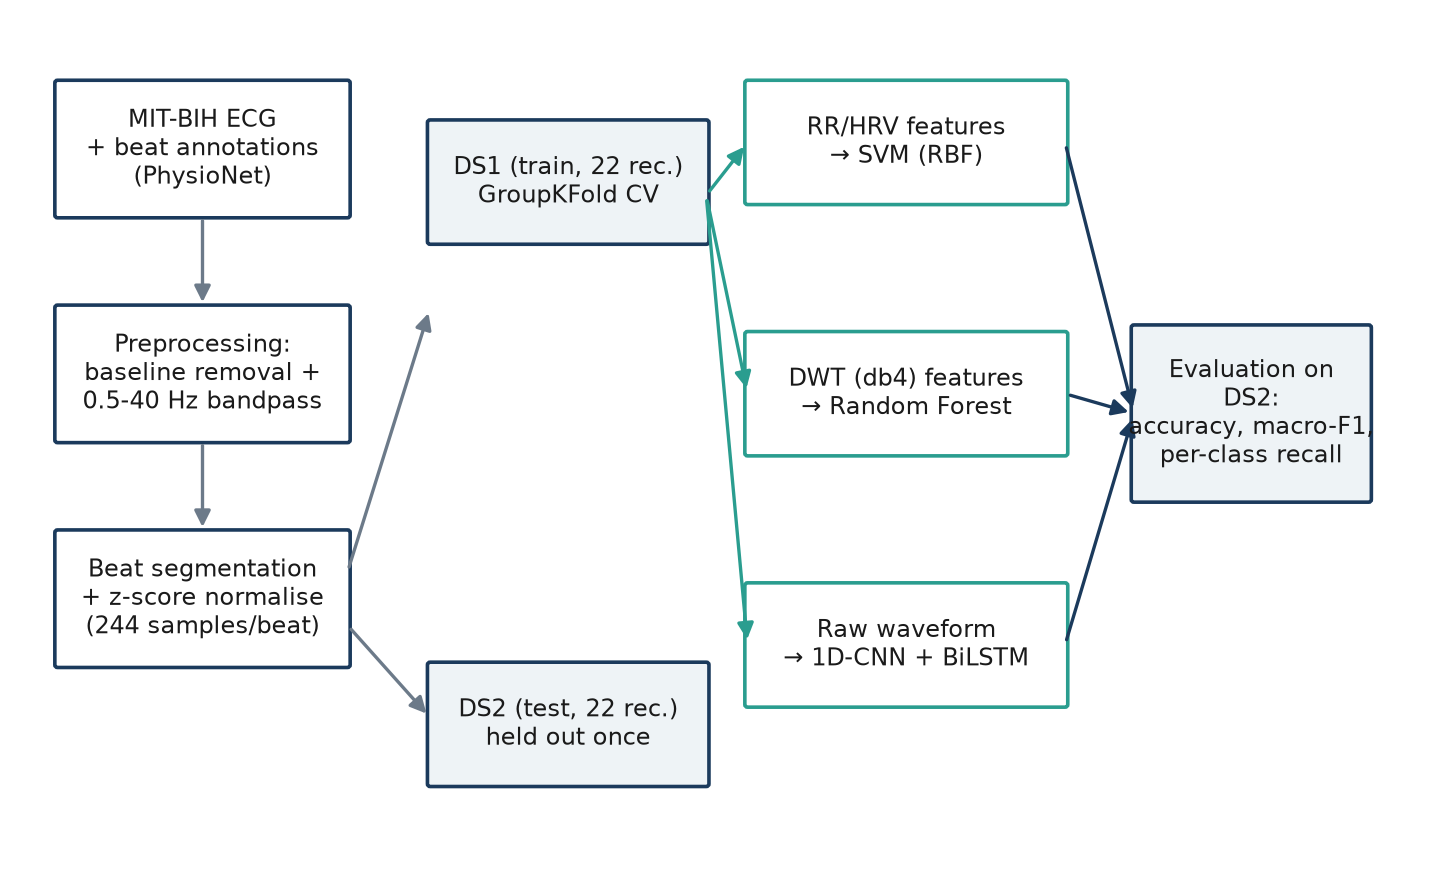
\includegraphics[width=\columnwidth]{figures/workflow.png}
\caption{Overall proposed ECG arrhythmia classification workflow. All three
approaches share identical preprocessing and the identical DS1/DS2 split;
they differ only in the feature representation fed to the classifier.}
\label{fig:workflow}
\end{figure}

\subsection{ECG Signal Preprocessing}

Each record's primary lead (MLII) is processed as follows.

\textit{Baseline wander removal.} A two-stage median filter removes slow
baseline drift without distorting the QRS complex, which a naive
high-pass filter can do:
\begin{equation}
x_{bl}[n] = \mathrm{median}_{w_2}\big(\mathrm{median}_{w_1}(x[n])\big)
\end{equation}
\begin{equation}
x_1[n] = x[n] - x_{bl}[n]
\end{equation}
with window lengths $w_1 \approx 200$~ms and $w_2 \approx 600$~ms at
360~Hz.

\textit{Bandpass filtering.} A 3rd-order Butterworth bandpass filter
(0.5--40~Hz), applied with zero-phase filtering (\texttt{filtfilt}) to
avoid phase distortion of the QRS complex, removes residual drift and
high-frequency noise:
\begin{equation}
X_2(f) = X_1(f)\cdot H_{BP}(f)
\end{equation}
where $H_{BP}(f) \neq 0$ for $f \in [0.5, 40]$~Hz.
The 40~Hz upper cutoff also attenuates 60~Hz mains interference (the
database was recorded in the United States), so a separate notch filter
is unnecessary.

\textit{Beat segmentation.} For each annotated R-peak at sample $r$, a
fixed window is extracted:
\begin{equation}
x_{beat} = x_2[\,r - 0.28\,f_s \; : \; r + 0.40\,f_s\,]
\end{equation}
giving $0.28\cdot360 + 0.40\cdot360 = 244$ samples per beat, covering the
QRS complex and T-wave. Windows that fall outside the recording, contain
non-finite values, or are flat ($\sigma \approx 0$, a recording artefact)
are dropped rather than zero-padded.

\textit{Normalisation.} Each beat is independently z-score normalised,
\begin{equation}
\hat{x}_{beat} = \frac{x_{beat} - \mu(x_{beat})}{\sigma(x_{beat})}
\end{equation}
so amplitude differences across patients, leads, and gain settings do not
dominate downstream features.

Across the 44 records, this pipeline yields 100{,}692 valid beats from
111{,}563 raw annotations (90.3\% beat-yield; the remainder are non-beat
markers or edge/invalid segments, Table~\ref{tab:dataset}).

\subsection{Approach 1: RR/HRV Features with SVM}

For each beat, the previous and next RR intervals are computed from the
\emph{filtered beat-annotation sequence} (rhythm/quality markers excluded
first, so timing is never computed against a non-beat marker):
\begin{equation}
RR_{prev} = \frac{r_i - r_{i-1}}{f_s}, \qquad RR_{next} = \frac{r_{i+1} - r_i}{f_s}
\end{equation}
From these, six features are derived (Table~\ref{tab:hrv}, Fig.~\ref{fig:hrv}):
mean RR, the RR ratio, a local successive-difference magnitude analogous
to RMSSD,
\begin{equation}
RMSSD_{local} = |RR_{next} - RR_{prev}|,
\end{equation}
and instantaneous heart rate, $HR = 60/RR_{mean}$.
Boundary beats (first/last in a record) have one missing neighbour
interval, imputed from the available one so no beat is discarded for
being at a record edge.

\begin{figure}[t]
\centering
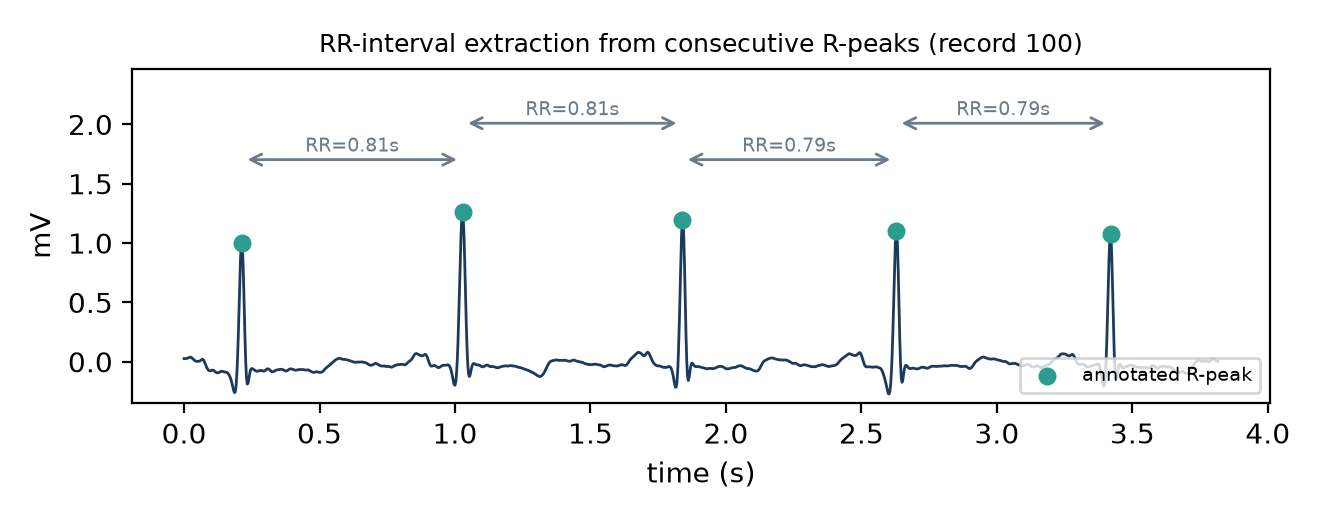
\includegraphics[width=\columnwidth]{figures/hrv_illustration.png}
\caption{RR-interval extraction from consecutive annotated R-peaks (record
100), the basis of the Approach 1 feature set.}
\label{fig:hrv}
\end{figure}

\begin{table}[t]
\caption{RR-Interval / HRV Feature Set (Approach 1)}
\label{tab:hrv}
\centering
\begin{tabular}{ll}
\toprule
\textbf{Feature} & \textbf{Definition} \\
\midrule
$RR_{prev}$ & interval to the preceding beat (s) \\
$RR_{next}$ & interval to the following beat (s) \\
$RR_{mean}$ & $(RR_{prev}+RR_{next})/2$ \\
$RR_{ratio}$ & $RR_{prev}/RR_{next}$ \\
$RR_{\Delta}$ & $|RR_{next}-RR_{prev}|$ (local RMSSD proxy) \\
$HR_{inst}$ & $60/RR_{mean}$ (instantaneous heart rate, bpm) \\
\bottomrule
\end{tabular}
\\[4pt]
\footnotesize All 6 features are standardised (zero mean, unit variance) before
the SVM. Missing boundary-beat intervals are imputed from the single
available neighbour (Section~IV-B).
\end{table}


Features are standardised and passed to a Support Vector
Machine with an RBF kernel,
\begin{equation}
f(x) = \mathrm{sign}\Big(\sum_{i} \alpha_i y_i \, K(x_i, x) + b\Big)
\end{equation}
\begin{equation}
K(x_i,x) = e^{-\gamma\|x_i - x\|^2}
\end{equation}
with \texttt{class\_weight="balanced"} to counteract class imbalance.
Hyperparameters $C \in \{1,10,100\}$ and $\gamma \in \{\text{scale},
0.01, 0.1\}$ are selected by grid search with 5-fold \texttt{GroupKFold}
cross-validation within DS1 (grouped by record), optimising macro-F1. The
RBF kernel's training cost grows super-linearly with sample count, so the
SVM is trained on a class-balanced subsample of DS1 capped at 4{,}000
beats/class (9{,}154 beats total after capping: N is downsampled from
45{,}847 to 4{,}000, while S, V, F, Q are kept in full since none exceeds
the cap); this is the one deliberate compute trade-off in this study and
is why Approaches 2 and 3 below, which scale better, are instead trained
on the full DS1 set.

\subsection{Approach 2: DWT Features with Random Forest}

The Discrete Wavelet Transform decomposes a beat into successive
approximation and detail coefficient bands via a quadrature mirror filter
pair $(h,g)$:
\begin{equation}
cA_{j+1}[k] = \sum_n h[n-2k]\,cA_j[n]
\end{equation}
\begin{equation}
cD_{j+1}[k] = \sum_n g[n-2k]\,cA_j[n]
\end{equation}
with $cA_0 = \hat{x}_{beat}$. This multi-resolution decomposition is
well suited to ECG beats because the QRS complex, P-wave, and T-wave
occupy different, localized frequency bands and timescales, which a
single global Fourier transform would blur together. A Daubechies-4
(\texttt{db4}) wavelet is used to level 4, yielding five coefficient bands
($cA_4, cD_4, cD_3, cD_2, cD_1$; Fig.~\ref{fig:dwt}). From each band $c$,
six statistics are computed: mean, standard deviation, minimum, maximum,
energy $E=\sum_k c[k]^2$, and Shannon entropy
\begin{equation}
H(c) = -\sum_k p_k \log p_k, \qquad p_k = \frac{c[k]^2}{\sum_j c[j]^2},
\end{equation}
giving a $5 \times 6 = 30$-dimensional feature vector (Table~\ref{tab:dwt}).

\begin{figure}[t]
\centering
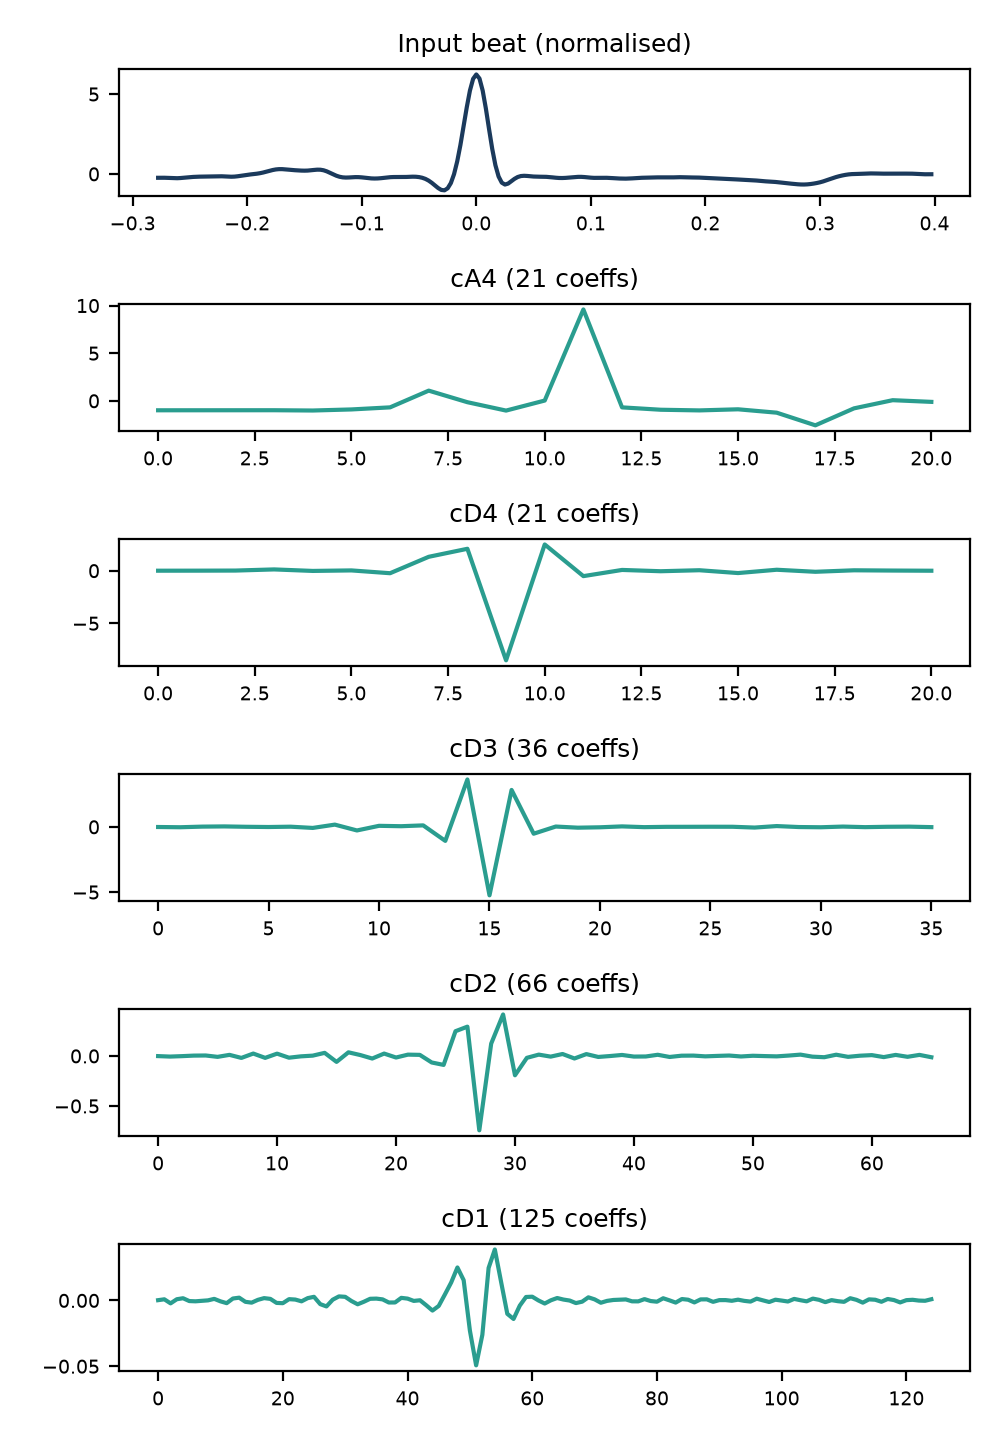
\includegraphics[width=\columnwidth]{figures/dwt_decomposition.png}
\caption{Level-4 \texttt{db4} wavelet decomposition of a real normal beat
into one approximation band ($cA_4$) and four detail bands
($cD_4$--$cD_1$), the basis of the Approach 2 feature set.}
\label{fig:dwt}
\end{figure}

\begin{table}[t]
\caption{Wavelet Feature Configuration (Approach 2)}
\label{tab:dwt}
\centering
\begin{tabular}{@{}p{0.34\columnwidth}p{0.56\columnwidth}@{}}
\toprule
\textbf{Parameter} & \textbf{Value} \\
\midrule
Wavelet & Daubechies-4 (\texttt{db4}) \\
Decomposition levels & 4 ($cA_4, cD_4, cD_3, cD_2, cD_1$) \\
Coefficient bands & 5 \\
Statistics per band & mean, std, min, max, energy, entropy \\
Total feature dimension & $5 \times 6 = 30$ \\
Classifier & Random Forest, \texttt{class\_weight="balanced"} \\
Hyperparameter grid & $n_{est}\!\in\!\{200,400\}$, depth$\in\{$None$,20\}$, leaf$\in\{1,3\}$ \\
\bottomrule
\end{tabular}
\end{table}


These features are passed to a Random Forest classifier with
\texttt{class\_weight="balanced"}; $n_{est} \in \{200,400\}$,
max depth $\in \{\text{None}, 20\}$, and min.\ leaf size $\in \{1,3\}$ are
selected by the same \texttt{GroupKFold} grid search as Approach 1, on
the \emph{full} DS1 training set.

\subsection{Approach 3: 1D-CNN + Bidirectional LSTM}

Approach 3 learns a representation directly from $\hat{x}_{beat}$ rather
than hand-crafting one. A 1D convolution over the beat,
\begin{equation}
z[k] = \mathrm{ReLU}\Big(\sum_{m} w[m]\, \hat{x}_{beat}[k+m] + b\Big),
\end{equation}
extracts local morphological patterns; two convolutional blocks
(16 then 32 filters, kernel sizes 7 and 5, each followed by ReLU and
max-pooling) progressively summarise the waveform (Table~\ref{tab:cnn},
Fig.~\ref{fig:cnnarch}). The resulting sequence is passed to a
bidirectional LSTM, which for each direction maintains
\begin{align}
f_t &= \sigma(W_f[h_{t-1},x_t]+b_f), &
i_t &= \sigma(W_i[h_{t-1},x_t]+b_i), \\
o_t &= \sigma(W_o[h_{t-1},x_t]+b_o), &
\tilde{c}_t &= \tanh(W_c[h_{t-1},x_t]+b_c), \\
c_t &= f_t \odot c_{t-1} + i_t \odot \tilde{c}_t, &
h_t &= o_t \odot \tanh(c_t),
\end{align}
and the forward/backward final hidden states are concatenated to capture
temporal structure in both directions across the beat. A dropout layer
($p=0.3$) regularises the 128-dimensional representation before a dense
layer and softmax,
\begin{equation}
P(y=k\mid x) = \frac{e^{z_k}}{\sum_{j=1}^{5} e^{z_j}}, \quad k \in \{N,S,V,F,Q\}.
\end{equation}

\begin{figure}[t]
\centering
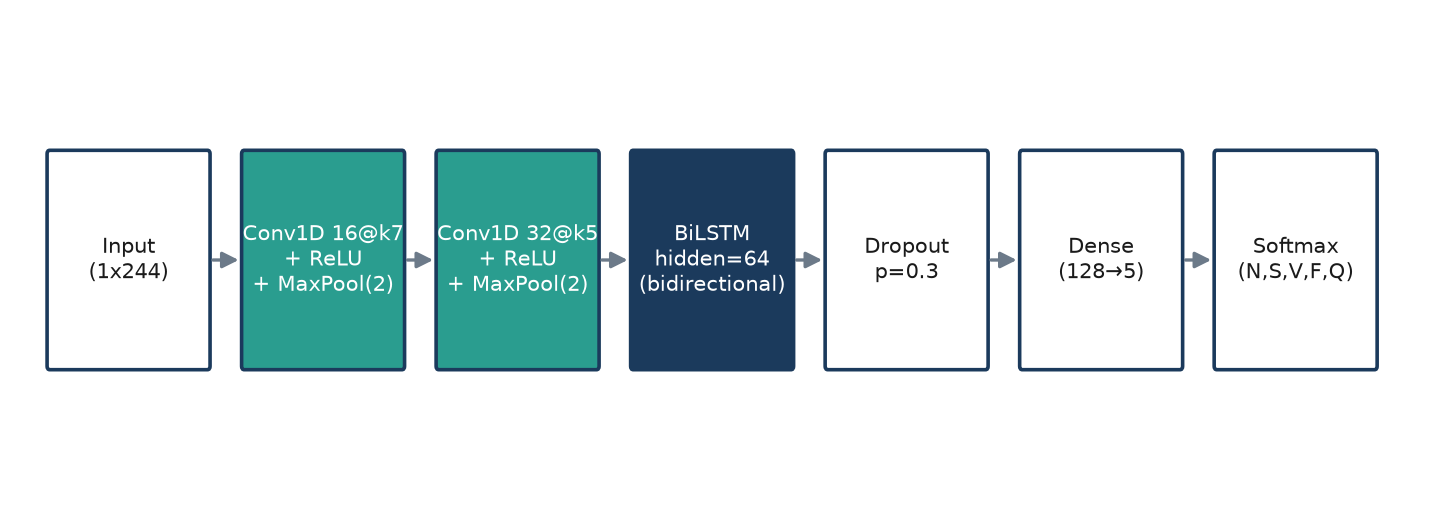
\includegraphics[width=\columnwidth]{figures/cnn_bilstm_architecture.png}
\caption{1D-CNN + BiLSTM architecture used in this study (matches the
implemented model exactly; see Table~\ref{tab:cnn}).}
\label{fig:cnnarch}
\end{figure}

\begin{table}[t]
\caption{1D-CNN + BiLSTM Architecture (Approach 3)}
\label{tab:cnn}
\centering
\begin{tabular}{lll}
\toprule
\textbf{Layer} & \textbf{Config.} & \textbf{Output shape} \\
\midrule
Input & raw normalised beat & $(1, 244)$ \\
Conv1D + ReLU & 16 filters, $k{=}7$, pad 3 & $(16, 244)$ \\
MaxPool1D & pool 2 & $(16, 122)$ \\
Conv1D + ReLU & 32 filters, $k{=}5$, pad 2 & $(32, 122)$ \\
MaxPool1D & pool 2 & $(32, 61)$ \\
BiLSTM & hidden 64, bidirectional & $(61, 128)$ \\
(last time step) & -- & $(128,)$ \\
Dropout & $p{=}0.3$ & $(128,)$ \\
Dense + Softmax & $128 \rightarrow 5$ & $(5,)$ \\
\bottomrule
\end{tabular}
\\[4pt]
\footnotesize Trained with Adam ($lr{=}10^{-3}$), batch size 128, up to 25
epochs with early stopping (patience 5) on DS1 validation macro-F1.
\end{table}


The network is trained with Adam ($lr=10^{-3}$), batch size 128, on the
full DS1 set further split 85\%/15\% by record (\texttt{GroupShuffleSplit})
into training and validation beats, with up to 25 epochs and early
stopping (patience 5) on \emph{validation macro-F1}. An initial
development run selected the checkpoint by validation loss with
uncapped inverse-frequency class weights; because class $Q$ has only
single-digit support in DS1, its inverse-frequency weight became large
enough to destabilise training (validation loss diverged while training
loss fell, and DS2 recall for the majority class $N$ collapsed to 0.38).
This was corrected, and is reported rather than hidden, by (i) capping
class weights at $10\times$ and (ii) selecting the checkpoint by
validation macro-F1 instead of validation loss, since loss computed over
a handful of $Q$ validation examples is too noisy to trust for model
selection. All results in Section~V use the corrected configuration.

\subsection{Experimental Setup}

Table~\ref{tab:setup} summarises the shared experimental configuration.
All three models use the identical DS1/DS2 split and the identical
preprocessed beats; hyperparameter selection for every model uses only
DS1 (via grouped cross-validation or a grouped validation split); DS2 is
touched exactly once, for the results reported in Section~V. A fixed
random seed (42) is used throughout for reproducibility. Training and
evaluation ran on a standard CPU (no GPU was used or required at this
model scale); wall-clock training time for the CNN-BiLSTM is not reported
precisely, since development was performed on a shared machine under
variable background load, but per-epoch compute cost was on the order of
tens of seconds, consistent with the model's small parameter count.

\begin{table}[t]
\caption{Experimental Configuration}
\label{tab:setup}
\centering
\begin{tabular}{@{}p{0.32\columnwidth}p{0.6\columnwidth}@{}}
\toprule
\textbf{Item} & \textbf{Value} \\
\midrule
Language / version & Python 3.12 \\
Core libraries & wfdb, NumPy, SciPy, scikit-learn, PyWavelets, PyTorch, pandas \\
Random seed & 42 (fixed across all models) \\
Train/test split & DS1 (22 rec.) / DS2 (22 rec.), patient-independent \\
Hyperparameter search & \texttt{GroupKFold} ($k{=}5$) within DS1 only \\
SVM training set & class-balanced DS1 subsample ($\leq$4,000/class) \\
RF, CNN-BiLSTM training set & full DS1 (51,001 beats) \\
CNN-BiLSTM val.\ split & 15\% of DS1 by record (\texttt{GroupShuffleSplit}) \\
Class imbalance handling & \texttt{class\_weight="balanced"} (SVM, RF); capped inverse-frequency weights, max $10\times$ (CNN) \\
Evaluation protocol & single evaluation on DS2, after hyperparameter selection \\
\bottomrule
\end{tabular}
\end{table}


\section{Experimental Results and Analysis}

\subsection{Dataset Class Distribution}

Fig.~\ref{fig:classdist} and Table~\ref{tab:dataset} show that class $N$
accounts for roughly 89\% of all beats in both DS1 and DS2, with $S$, $V$,
$F$, and especially $Q$ far rarer. This imbalance is the central reason
accuracy alone cannot meaningfully rank the three approaches below: a
model predicting $N$ for every beat would already score close to 0.89
accuracy while being clinically useless.

\begin{figure}[t]
\centering
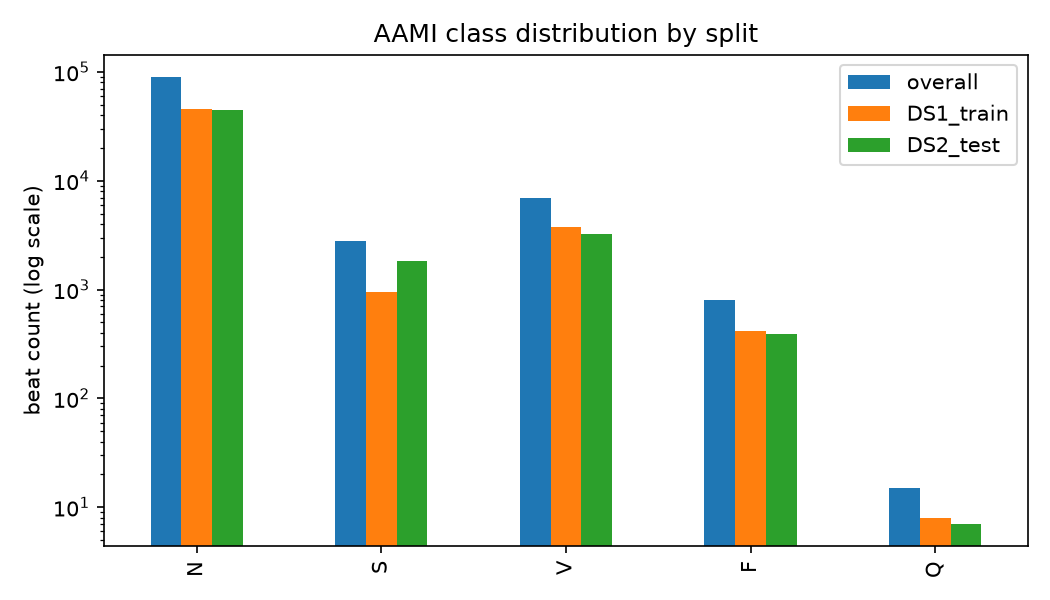
\includegraphics[width=\columnwidth]{figures/class_distribution.png}
\caption{AAMI class distribution (log scale) for the overall dataset, DS1,
and DS2, confirming consistent, severe imbalance across the split.}
\label{fig:classdist}
\end{figure}

\begin{figure}[t]
\centering
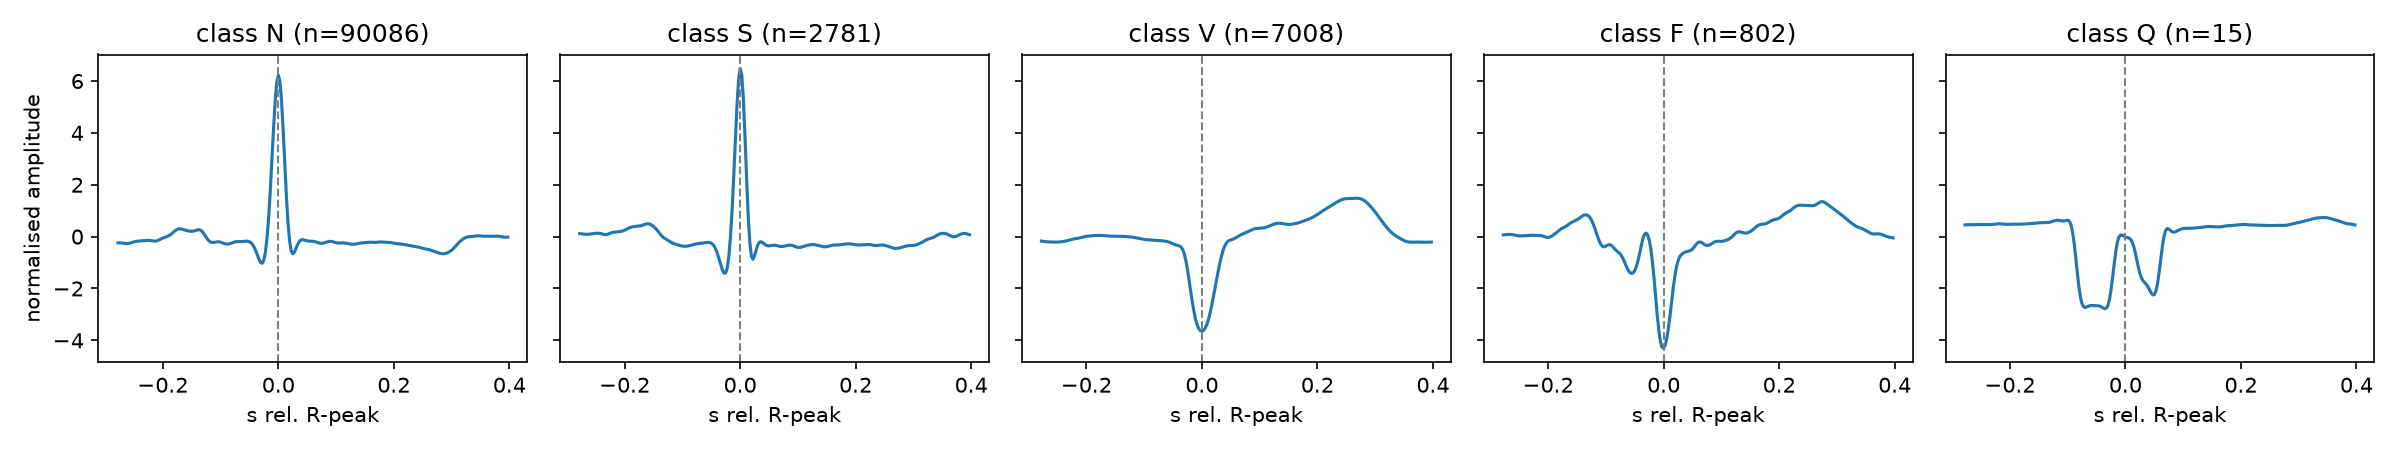
\includegraphics[width=\columnwidth]{figures/sample_beats.png}
\caption{Representative segmented, normalised beats for each AAMI class
(record-level examples from the actual processed dataset).}
\label{fig:samplebeats}
\end{figure}

\subsection{Overall Performance Comparison}

Table~\ref{tab:performance} and Fig.~\ref{fig:modelcomp} report accuracy,
macro-F1, weighted-F1, and per-class precision/recall for all three
models on the untouched DS2 test set. No hyperparameter in any model was
selected using DS2.

\begin{table*}[t]
\caption{Comparative Performance of the Three Approaches on the DS2 Test Set (49{,}691 beats)}
\label{tab:performance}
\centering
\footnotesize
\begin{tabular}{lccccccccccccc}
\toprule
& & & & \multicolumn{2}{c}{N} & \multicolumn{2}{c}{S} & \multicolumn{2}{c}{V} & \multicolumn{2}{c}{F} & \multicolumn{2}{c}{Q} \\
\cmidrule(lr){5-6}\cmidrule(lr){7-8}\cmidrule(lr){9-10}\cmidrule(lr){11-12}\cmidrule(lr){13-14}
\textbf{Model} & \textbf{Acc.} & \textbf{Macro-F1} & \textbf{W.-F1} & P & R & P & R & P & R & P & R & P & R \\
\midrule
SVM (RR/HRV)         & 0.789 & \textbf{0.362} & 0.839 & 0.967 & 0.814 & 0.111 & 0.046 & 0.682 & 0.851 & 0.053 & \textbf{0.943} & 0.001 & 0.143 \\
Random Forest (DWT)  & \textbf{0.884} & 0.334 & \textbf{0.882} & 0.942 & \textbf{0.932} & 0.074 & 0.006 & 0.638 & \textbf{0.835} & 0.000 & 0.000 & 0.000 & 0.000 \\
CNN-BiLSTM            & 0.449 & 0.183 & 0.570 & 0.957 & 0.460 & 0.037 & 0.127 & 0.151 & 0.539 & 0.000 & 0.010 & 0.000 & 0.000 \\
\bottomrule
\end{tabular}
\\[4pt]
\footnotesize P = precision, R = recall, W.-F1 = weighted-F1. ROC-AUC
(macro, one-vs-rest): SVM 0.812, RF 0.730, CNN-BiLSTM 0.563. Q has only 7
test beats (Section III); its metrics are not statistically reliable.
\end{table*}


\begin{figure}[t]
\centering
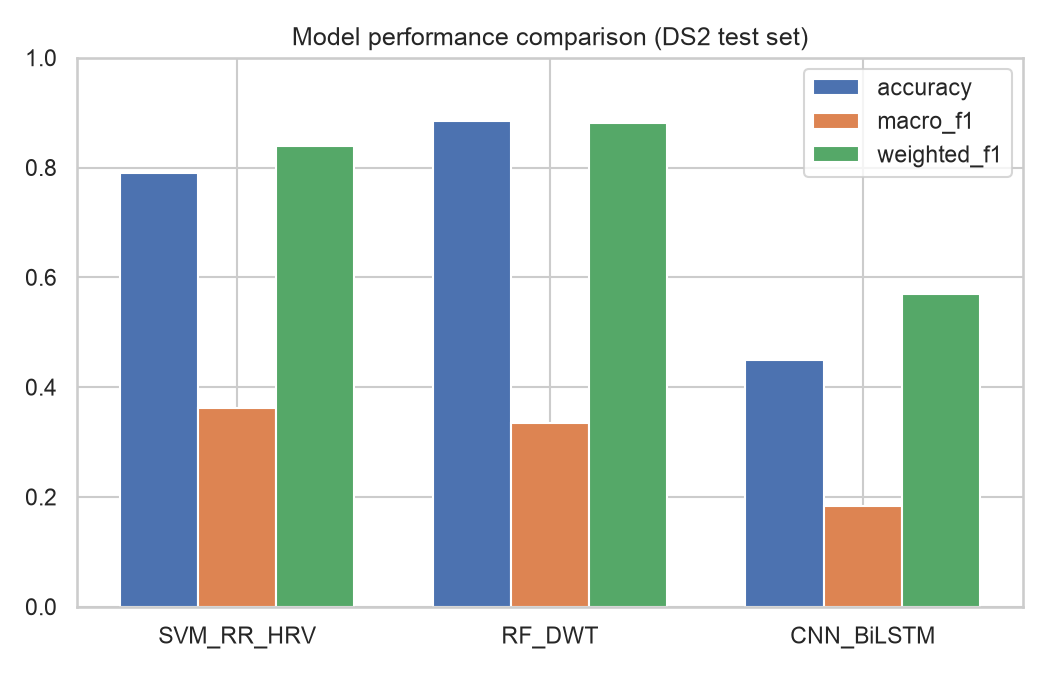
\includegraphics[width=\columnwidth]{figures/model_comparison.png}
\caption{Comparative model performance (accuracy, macro-F1, weighted-F1)
on the DS2 test set.}
\label{fig:modelcomp}
\end{figure}

Random Forest achieves the highest accuracy (0.884) and weighted-F1
(0.882); the SVM achieves the highest macro-F1 (0.362) and ROC-AUC
(0.812); the CNN-BiLSTM, in this configuration, trails both on every
aggregate metric. These three metrics do not agree on a single "best"
model, which is itself the main empirical finding of this study and is
discussed in Section~VI.

\subsection{Per-Class Analysis and Confusion Matrices}

Fig.~\ref{fig:cmsvm}--\ref{fig:cmcnn} show the DS2 confusion matrix for
each model, and Fig.~\ref{fig:perclassf1} compares per-class F1 directly.

\begin{figure}[t]
\centering
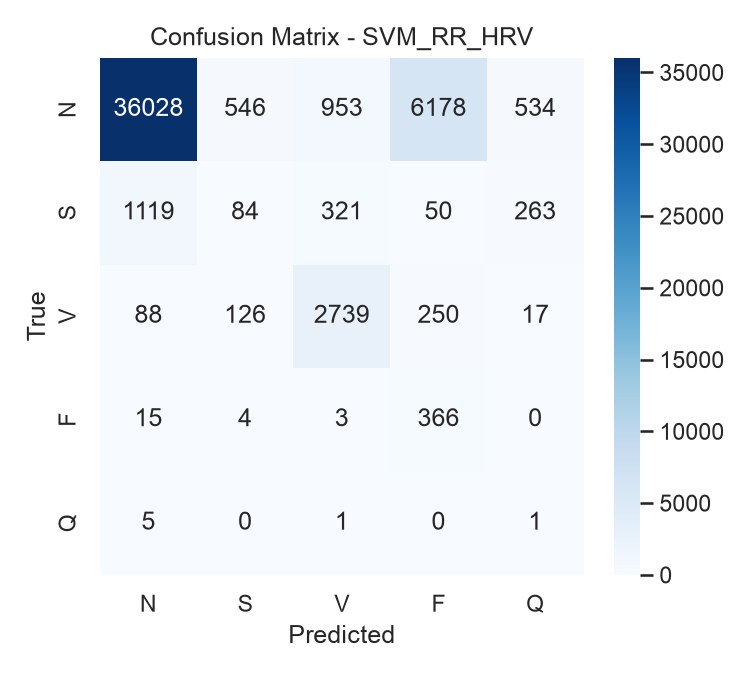
\includegraphics[width=\columnwidth]{figures/confusion_matrix_svm.png}
\caption{Confusion matrix of the SVM (RR/HRV) classifier on DS2.}
\label{fig:cmsvm}
\end{figure}

\begin{figure}[t]
\centering
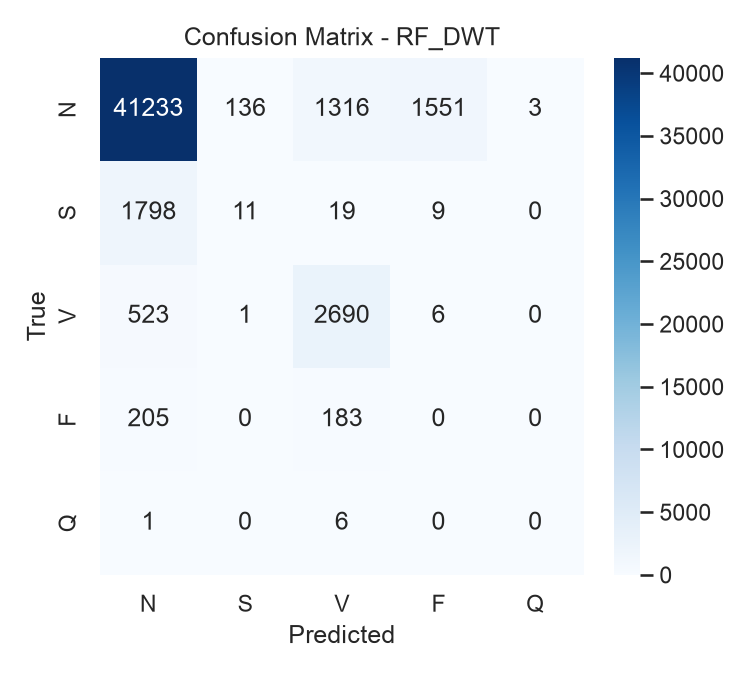
\includegraphics[width=\columnwidth]{figures/confusion_matrix_rf.png}
\caption{Confusion matrix of the Random Forest (DWT) classifier on DS2.}
\label{fig:cmrf}
\end{figure}

\begin{figure}[t]
\centering
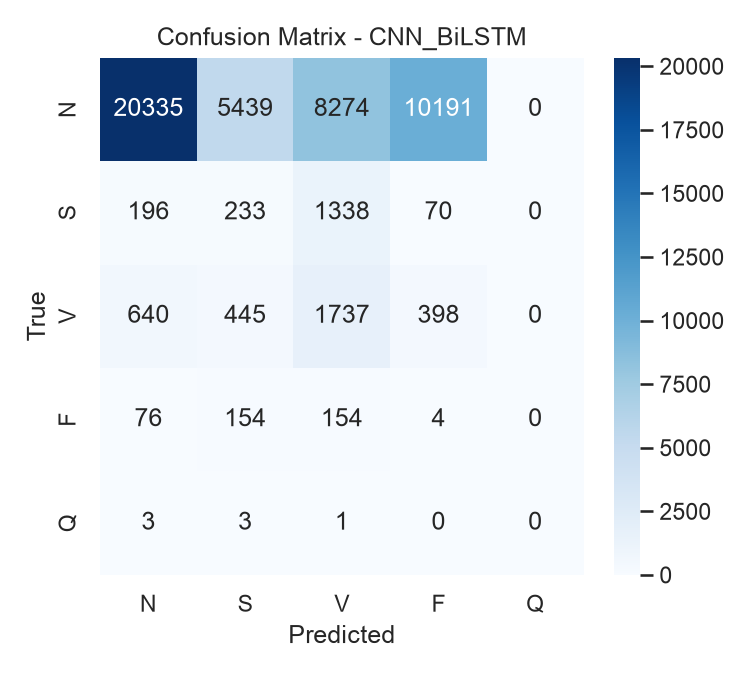
\includegraphics[width=\columnwidth]{figures/confusion_matrix_cnn_bilstm.png}
\caption{Confusion matrix of the CNN-BiLSTM classifier on DS2.}
\label{fig:cmcnn}
\end{figure}

\begin{figure}[t]
\centering
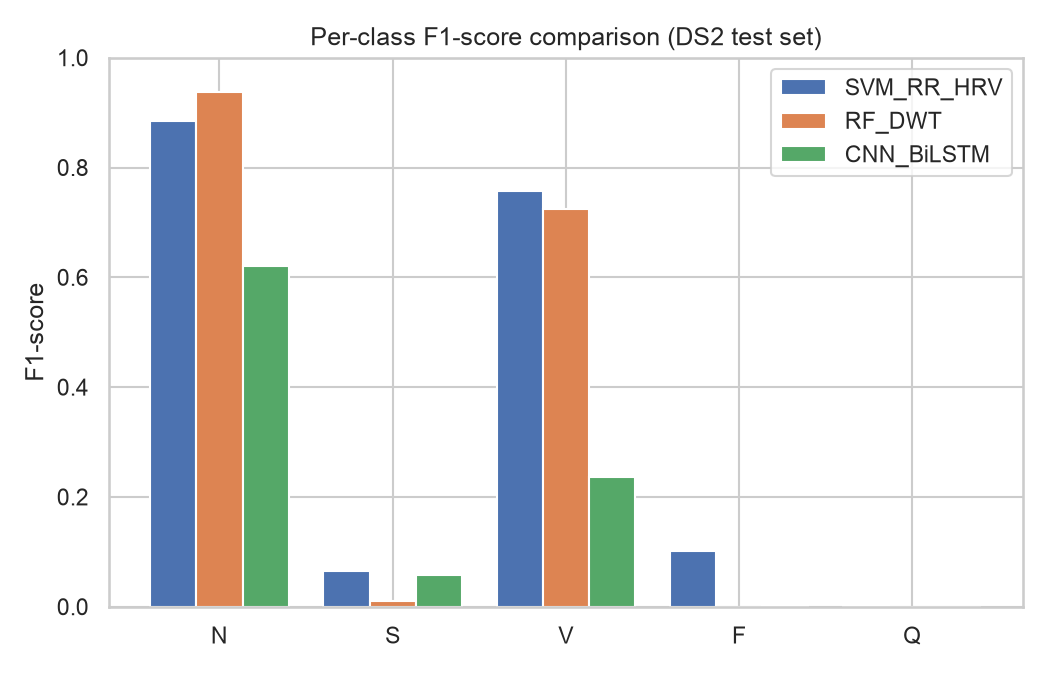
\includegraphics[width=\columnwidth]{figures/per_class_f1_comparison.png}
\caption{Per-class F1-score comparison across the three models on DS2.}
\label{fig:perclassf1}
\end{figure}

Class $N$ is handled well by all three (F1 0.884--0.937), except the
CNN-BiLSTM (F1 0.621, recall 0.460), whose capped class weighting
deliberately trades some $N$ recall for minority-class recall. Class $V$
is the best-handled minority class for every model (F1 0.724--0.757),
consistent with ventricular ectopic beats having a relatively distinct
waveform morphology that both wavelet statistics and learned
convolutional filters can capture. Class $S$ is poorly handled by all
three models (F1 $\leq$ 0.065), indicating that none of the three feature
representations used here cleanly separates supraventricular ectopic
beats from normal beats -- a known difficulty in the inter-patient
literature, since $S$ beats can closely resemble $N$ beats morphologically
and their timing signature is less distinctive than $V$'s. Class $F$
shows a striking divergence: the SVM achieves recall 0.943 (it rarely
misses a true fusion beat) but precision only 0.053 (it also mislabels
many non-$F$ beats as $F$), while Random Forest and CNN-BiLSTM essentially
never predict $F$ correctly (F1 $\approx$ 0). This suggests RR timing
alone is unusually (over-)sensitive to the fusion-beat pattern, while
wavelet statistics and the compact learned representation do not isolate
it. Class $Q$, with only 7 test beats, is not reliably measured by any
model and is excluded from substantive comparison.

\subsection{CNN-BiLSTM Training Behaviour}

Fig.~\ref{fig:traincurves} shows training/validation loss and validation
macro-F1 across epochs for the corrected configuration (Section IV-D).
Training loss decreases steadily while validation loss is noisier but
does not diverge, and validation macro-F1 plateaus around 0.29--0.31
before early stopping triggers at epoch 8, substantially lower than its
performance on DS2 (macro-F1 0.183) -- itself evidence of harder
generalisation to genuinely unseen patients than to the held-out-by-record
DS1 validation split, which is drawn from the same 22 training records'
general population characteristics.

\begin{figure}[t]
\centering
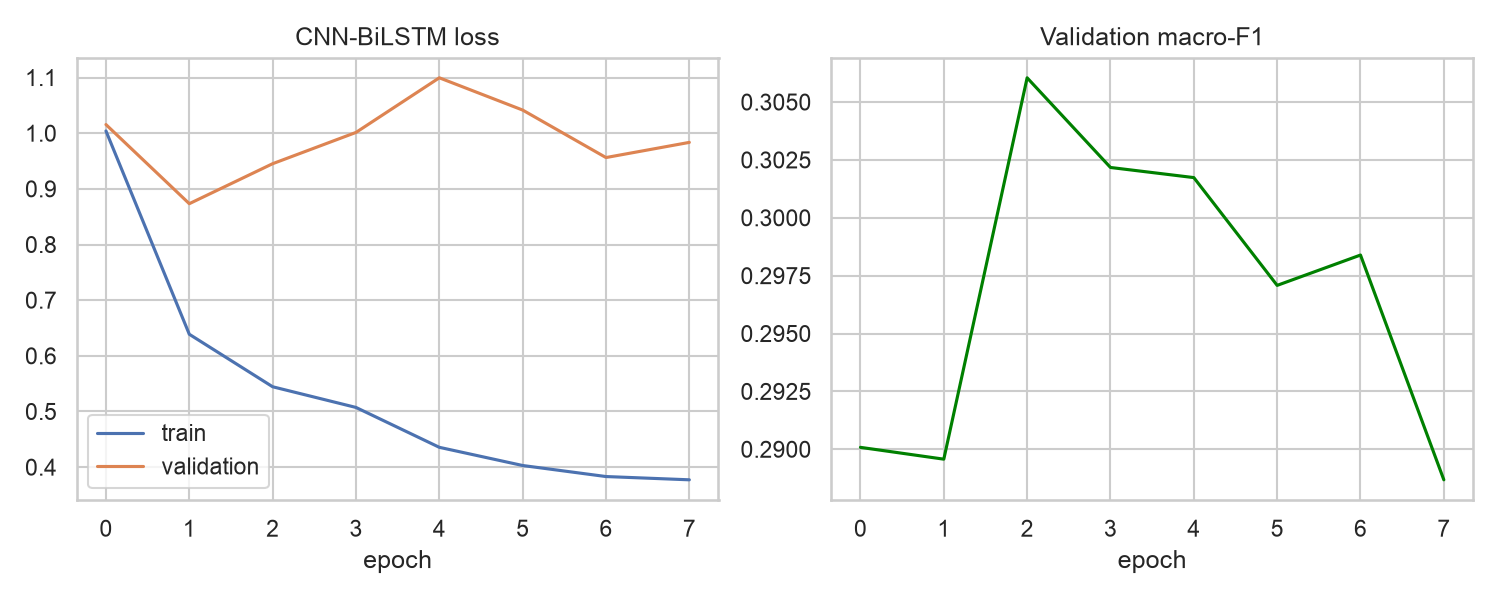
\includegraphics[width=\columnwidth]{figures/training_curves.png}
\caption{CNN-BiLSTM training/validation loss and validation macro-F1
across training epochs (corrected class-weighting configuration).}
\label{fig:traincurves}
\end{figure}

\section{Discussion}

\textbf{RR/HRV features (Approach 1).} The strength of this approach is
that RR timing is largely patient-invariant -- a premature beat shortens
the preceding interval similarly across individuals -- which plausibly
explains its best-in-class macro-F1 and ROC-AUC, and its unusually strong
fusion-beat recall. Its weakness is equally clear: with no waveform
information at all, it cannot distinguish classes that share similar
timing but different morphology, visible in its very low $F$ precision
(many false fusion-beat predictions) and weak $S$ recall.

\textbf{Wavelet features (Approach 2).} DWT statistics capture
localized, multi-scale morphological structure and, combined with a
Random Forest, give the best raw accuracy and weighted-F1 in this study
-- largely by being very good at the dominant class $N$. However, its
near-zero recall on $S$ and complete failure on $F$ and $Q$, despite
class-balanced training, suggest that a single beat's wavelet-coefficient
statistics do not carry enough class-discriminative signal for these
rarer categories once evaluated on truly unseen patients, even though
in-sample (DS1 cross-validation) performance is comparable to the SVM's.

\textbf{CNN-BiLSTM (Approach 3).} The hybrid deep model underperforms
both classical approaches here. We attribute this to the combination of
(i) an intentionally compact architecture and short training schedule
within this project's compute budget, well below what
Acharya et al.~\cite{acharya2017deep} and
Liu et al.~\cite{liu2019attention} used to report substantially higher
accuracy; (ii) no explicit timing (RR-interval) input, so the network
must infer temporal context from waveform shape alone; and (iii) the
capped class-weighting scheme, which, while necessary to avoid the
training instability documented in Section IV-D, further trades $N$
recall for minority-class sensitivity that the model is not yet capable
of exploiting well. This is a genuine limitation of the present
configuration, not evidence that CNN-BiLSTM architectures are
inherently weaker for this task.

\textbf{Computational and practical implications.} The SVM and Random
Forest are each trained and evaluated in under a minute per run on a
single CPU core once beats are cached, and require no specialised
hardware. The CNN-BiLSTM, despite its small size, has a materially higher
engineering and tuning cost (architecture search, class-weight tuning,
longer training loops) for a worse outcome in this configuration --
a practically relevant trade-off for a resource-constrained deployment,
though it does not rule out a larger or better-tuned deep model
eventually surpassing the classical approaches (Section VII).

\textbf{Generalisation to unseen patients.} The gap between DS1
cross-validation/validation performance and DS2 test performance,
visible for all three models but most pronounced for the CNN-BiLSTM
(Section V-D), underscores why the inter-patient split is not an
optional methodological detail: it is the difference between an
optimistic, patient-memorising estimate and a realistic one.

\textbf{Limitations.} This study uses a single lead (MLII), a
45-year-old research database recorded from 47 subjects, and does not
evaluate on any second database; results should not be extrapolated to
modern recording hardware or different patient populations. Class $Q$'s
single-digit support (Table~\ref{tab:dataset}) means its reported metrics
are illustrative only. Finally, this system is an offline, retrospective
research prototype: it is not a clinically validated diagnostic or
real-time monitoring tool, and none of the results above should be read
as a clinical performance claim.

\section{Conclusion and Future Scope}

This paper compared three heartbeat classification approaches --
RR/HRV features with SVM, DWT features with Random Forest, and a 1D-CNN +
BiLSTM trained on raw waveforms -- under one identical, patient-independent
evaluation protocol on the MIT-BIH Arrhythmia Database. No single model
dominates every metric: Random Forest leads on accuracy and weighted-F1,
the SVM leads on macro-F1 and ROC-AUC, and the compact CNN-BiLSTM trails
both in this configuration. The most important conclusion is methodological
rather than purely about which model "wins": under severe class imbalance
and a genuine inter-patient evaluation, accuracy is an unreliable ranking
criterion, and a model's apparent strength (e.g. the SVM's fusion-beat
recall, or the Random Forest's overall accuracy) can mask a serious
weakness (e.g. near-zero precision, or near-zero recall on other minority
classes) that only per-class, inter-patient evaluation reveals.

Future work should pursue: (i) larger and more diverse ECG datasets, and
external validation on a second database (e.g. INCART or PTB-XL) to test
cross-database, not just cross-patient, generalisation; (ii) improved
minority-class detection, for example by combining RR-interval input with
learned waveform features in a single model, or through
imbalance-aware losses less prone to the instability documented here;
(iii) a larger, longer-trained CNN-BiLSTM with a proper learning-rate
schedule, to test whether the gap to classical methods closes or reverses
with greater capacity; (iv) explainability methods (e.g. attention maps
or SHAP values) to make per-class failure modes interpretable to a
clinical reviewer; and (v) only after such validation, carefully
controlled, prospectively validated real-time ECG monitoring studies --
which remain well outside the scope of this retrospective, offline
comparison.

\section*{Acknowledgment}
The MIT-BIH Arrhythmia Database is provided by PhysioNet
\cite{goldberger2000physiobank}, originally compiled by the Beth Israel
Hospital Arrhythmia Laboratory~\cite{moody2001impact}.

\bibliographystyle{IEEEtran}
\bibliography{references}

\end{document}
